% !TEX root=index.tex
\chapter{Analisi dei risultati}\label{ch:cap_5}
	Gli esperimenti sono stati condotti con dei dati di istanza che fossero il più possibile realistici. Sono state analizzate tre classi di problemi: a flotta unitaria e senza time window, a flotta multipla senza time window ed infine a flotta multipla con time window. \\*
	Le seguenti istanze sono state risolte utilizzando un laptop equipaggiato con una CPU Intel i3 quadcore a 2,67GHz e 4Gb di RAM (non più di 10 minuti di calcolo ad istanza). È stata utilizzata la versione 12.6 di CPLEX mantenendo le impostazioni di default per la risoluzione di problemi di PLIM (\emph{Programmazione Lineare Intera Mista}).

	\section{Presentazione dati statici ed ipotesi esemplificative}
	\label{sec:il_linguaggio_di_modellazione_ampl}
		Qui di seguito viene riportata una tabella (tabella \ref{table:parametri statici}) riassuntiva con tutti i valori dei parametri statici utilizzati nella formulazione delle istanze del modello:

		\begin{table}[]
			\centering
			\begin{tabular}{@{}clc@{}}
					\toprule
					Notazione    & \multicolumn{1}{c}{Descrizione}                  & Valore \\ \midrule
					$g$          & costante gravitazionale (m/$s^2$)                & 9,81   \\
					$\rho$       & densità dell'aria (kg/$m^3$)                     & 1,255  \\
					$c_f$        & costo del carburante (€/l)                       & 1,20   \\
					$c_e$        & costo delle emissioni $CO_2$ (€/kg)              & 0,034  \\
					$U_{diesel}$ & energia intrinseca in 1 litro di carburante (MJ) & 36,4   \\
					$f_e$        & emissioni di $CO_2$ (kg/l)                       & 2,65   \\
					$\eta$       & efficienza del motore diesel (\%)                & 45     \\
					$M$          & massa a pieno carico del veicolo (kg)            & 8000   \\
					$w$          & massa a vuoto del veicolo (kg)                   & 4400   \\
					$C_r$        & coefficiente di resistenza al rotolamento        & 0,02   \\
					$C_d$        & resistenza alla penetrazione dell'aria           & 0,7    \\
					$A$          & area frontale del veicolo ($m^2$)                & 7      \\
					$p$          & salario dell'autista (€/h)                       & 8,5    \\ \bottomrule
			\end{tabular}
			\caption{Parametri dei veicoli e delle emissioni}
			\label{table:parametri statici}
		\end{table}

		Per ciò che riguarda le pendenze dei tratti stradali, queste sono state approssimate tutte a 0.
		Le motivazioni sono sostanzialmente due:

		\begin{itemize}
			\item raccogliere i dati riguardanti le quote dei tratti di strada che collegano i vari nodi è un’operazione lunga, la cui complessità esplode molto velocemente all’aumentare dei nodi.
			\item i risultati espressi nel paper \cite{Laporte11} si riferiscono tutti ad istanze di problemi valutate facendo la medesima assunzione.
		\end{itemize}

		Inoltre, i \emph{service time} di tutti i nodi, per questioni semplificative, sono stati fissati tutti quanti a 30minuti. Questa assunzione non lede in alcun modo la generalità della trattazione.

	\section{Risultati dell’istanza con un veicolo e senza time window}
	\label{sec:istanza_singolo_veicolo_no_time_window}
		Sono state prese in considerazione le seguenti città inglesi: Stokeontrent,	Derby, Eastwood, Mansfield,	Sheffield, Stockport, Preston, Liverpool, Chester e Warrington. In tabella \ref{table:distanza_citta} sono riportate le distanze da una città all’altra.

		\vspace{0.5cm}
		\begin{table}[H]
			\centering
			\resizebox{\columnwidth}{!}{
			\begin{tabular}{ @{} r c c c c c c c c c c @{} }
				\toprule 

				& Stoke-on-Trent & Derby  & Eastwood & Mansfield & Sheffield & Stockport & Preston & Liverpool & Chester & Warrington \\ 

				\midrule
				
				\multicolumn{1}{b{3cm}|}{Stoke-on-Trent} & -            & 56400  & 80200    & 90400     & 76300     & 69900     & 105000  & 91000     & 72000   & 59600      \\
				\multicolumn{1}{b{1.8cm}|}{Derby}        & 56400        & -      & 18900    & 37500     & 65200     & 86400     & 148000  & 136000    & 98500   & 104000     \\
				\multicolumn{1}{b{1.8cm}|}{Eastwood}     & 80200        & 18900  & -        & 19400     & 51200     & 85900     & 178000  & 143000    & 102000  & 116000     \\
				\multicolumn{1}{b{1.8cm}|}{Mansfield}    & 90400        & 37500  & 19400    & -         & 38700     & 80100     & 192000  & 173000    & 108000  & 115000     \\
				\multicolumn{1}{b{1.8cm}|}{Sheffield}    & 76300        & 65200  & 51200    & 38700     & -         & 59400     & 119000  & 129000    & 60900   & 94400      \\
				\multicolumn{1}{b{1.8cm}|}{Stockport}    & 69900        & 86400  & 85900    & 80100     & 59400     & -         & 68200   & 67100     & 10700   & 37000      \\
				\multicolumn{1}{b{1.8cm}|}{Preston}      & 105000       & 148000 & 178000   & 192000    & 119000    & 68200     & -       & 54800     & 53400   & 49900      \\
				\multicolumn{1}{b{1.8cm}|}{Liverpool}    & 91000        & 136000 & 143000   & 173000    & 129000    & 67100     & 54800   & -         & 55700   & 29500      \\
				\multicolumn{1}{b{1.8cm}|}{Chester}      & 60900        & 146000 & 143000   & 169000    & 122000    & 82200     & 91400   & 29000     & -       & 34900      \\
				\multicolumn{1}{b{1.8cm}|}{Warrington}   & 59600        & 104000 & 116000   & 115000    & 94400     & 37000     & 49900   & 29500     & 32700   & -          \\ \bottomrule
			\end{tabular}}
			\caption{Distanza tra le città (in metri)}
			\label{table:distanza_citta}
		\end{table}

		Si consideri inoltre che si ha a disposizione un solo veicolo che, a partire dalla città di  Stockport, deve visitare tutte le altre e farvi ritorno, minimizzando il costo complessivo del problema di PRP associato.

		\begin{table}[H]
			\tiny
			\centering
			\label{table:instance_1_x}
			\begin{tabular}{rcccccccccc}
				\toprule
				& \rot{Chester} & \rot{Derby} & \rot{Eastwood} & \rot{Liverpool} & \rot{Mansfield} & \rot{Preston} & \rot{Sheffield} & \rot{\emph{Stockport}} & \rot{Stoke on Trent} & \rot{Warrington} \\

				\midrule

				Chester & 0 & 0 & 0 & \cellcolor{blue!25}1 & 0 & 0 & 0 & 0 & 0 & 0 \\
				Derby & 0 & 0 & \cellcolor{blue!25}1 & 0 & 0 & 0 & 0 & 0 & 0 & 0 \\
				Eastwood & 0 & 0 & 0 & 0 & \cellcolor{blue!25}1 & 0 & 0 & 0 & 0 & 0 \\
				Liverpool & 0 & 0 & 0 & 0 & 0 & \cellcolor{blue!25}1 & 0 & 0 & 0 & 0 \\
				Mansfield & 0 & 0 & 0 & 0 & 0 & 0 & \cellcolor{blue!25}1 & 0 & 0 & 0 \\
				Preston & 0 & 0 & 0 & 0 & 0 & 0 & 0 & 0 & 0 & \cellcolor{blue!25}1 \\
				Sheffield & 0 & 0 & 0 & 0 & 0 & 0 & 0 & \cellcolor{blue!25}1 & 0 & 0 \\
				\emph{Stockport} & \cellcolor{blue!25}1 & 0 & 0 & 0 & 0 & 0 & 0 & 0 & 0 & 0 \\
				Stoke on Trent & 0 & \cellcolor{blue!25}1 & 0 & 0 & 0 & 0 & 0 & 0 & 0 & 0 \\
				Warrington & 0 & 0 & 0 & 0 & 0 & 0 & 0 & 0 & \cellcolor{blue!25}1 & 0 \\

				\bottomrule
			\end{tabular}
			\label{table:instance_1_xij}
			\caption{Valori degli $x_{ij}$ per l'istanza con un veicolo senza time window}
		\end{table}


		\begin{table}[H]
			\tiny
			\centering
			\begin{tabular}{rcccccccccc}

				\toprule
				& \rot{Chester} & \rot{Derby} & \rot{Eastwood} & \rot{Liverpool} & \rot{Mansfield} & \rot{Preston} & \rot{Sheffield} & \rot{Stockport} & \rot{Stoke on Trent} & \rot{Warrington} \\

				\midrule

				Chester & 0 & 0 & 0 & 1800 & 0 & 0 & 0 & 0 & 0 & 0 \\
				Derby & 0 & 0 & 800 & 0 & 0 & 0 & 0 & 0 & 0 & 0\\
				Eastwood & 0 & 0 & 0 & 0 & 600 & 0 & 0 & 0 & 0 & 0\\
				Liverpool & 0 & 0 & 0 & 0 & 0 & 1600 & 0 & 0 & 0 & 0\\
				Mansfield & 0 & 0 & 0 & 0 & 0 & 0 & 400 & 0 & 0 & 0\\
				Preston & 0 & 0 & 0 & 0 & 0 & 0 & 0 & 0 & 0 & 1400 \\
				Sheffield & 0 & 0 & 0 & 0 & 0 & 0 & 0 & 200 & 0 & 0\\
				Stockport & 2000 & 0 & 0 & 0 & 0 & 0 & 0 & 0 & 0 & 0 \\
				Stoke on Trent & 0 & 1000 & 0 & 0 & 0 & 0 & 0 & 0 & 0 & 0 \\
				Warrington & 0 & 0 & 0 & 0 & 0 & 0 & 0 & 0 & 1200 & 0\\
				\bottomrule
			\end{tabular}
			\label{table:instance_1_f}
			\caption{Quantità di merce traportata $f_{ij}$ per l'istanza con un veicolo senza time window}
		\end{table}


		\begin{table}[H]
			\tiny
			\centering
			\begin{tabular}{rcccccccccc}

				\toprule
				& \rot{Chester} & \rot{Derby} & \rot{Eastwood} & \rot{Liverpool} & \rot{Mansfield} & \rot{Preston} & \rot{Sheffield} & \rot{Stockport} & \rot{Stoke on Trent} & \rot{Warrington} \\

				\midrule

				Chester & 0 & 0 & 0 & 1 & 0 & 0 & 0 & 0 & 0 & 0 \\
				Derby & 0 & 0 & 1 & 0 & 0 & 0 & 0 & 0 & 0 & 0 \\
				Eastwood & 0 & 0 & 0 & 0 & 1 & 0 & 0 & 0 & 0 & 0 \\
				Liverpool & 0 & 0 & 0 & 0 & 0 & 1 & 0 & 0 & 0 & 0 \\
				Mansfield & 0 & 0 & 0 & 0 & 0 & 0 & 1 & 0 & 0 & 0 \\
				Preston & 0 & 0 & 0 & 0 & 0 & 0 & 0 & 0 & 0 & 1 \\
				Sheffield & 0 & 0 & 0 & 0 & 0 & 0 & 0 & 1 & 0 & 0 \\
				Stockport & 1 & 0 & 0 & 0 & 0 & 0 & 0 & 0 & 0 & 0 \\
				Stoke on Trent & 0 & 1 & 0 & 0 & 0 & 0 & 0 & 0 & 0 & 0 \\
				Warrington & 0 & 0 & 0 & 0 & 0 & 0 & 0 & 0 & 1 & 0 \\
				\bottomrule
			\end{tabular}
			\label{table:instance_1_z_1}
			\caption{Valori di $z_{ij}^1$ per l'istanza con un veicolo senza time window}
		\end{table}	
		% \begin{minipage}[t]{0.49\textwidth}
		% 	\begin{table}[H]
		% 	\tiny
		% 	\centering
		% 	\label{table:instance_1_z_2}
		% 	\begin{tabular}{p{1cm} cccccccccc}

		% 		\toprule
		% 		& \rot{Chester} & \rot{Derby} & \rot{Eastwood} & \rot{Liverpool} & \rot{Mansfield} & \rot{Preston} & \rot{Sheffield} & \rot{Stockport} & \rot{Stoke on Trent} & \rot{Warrington} \\

		% 		\midrule

		% 		Chester & 0 & 0 & 0 & 0 & 0 & 0 & 0 & 0 & 0 & 0 \\
		% 		Derby & 0 & 0 & 0 & 0 & 0 & 0 & 0 & 0 & 0 & 0 \\
		% 		Eastwood & 0 & 0 & 0 & 0 & 0 & 0 & 0 & 0 & 0 & 0 \\
		% 		Liverpool & 0 & 0 & 0 & 0 & 0 & 0 & 0 & 0 & 0 & 0 \\
		% 		Mansfield & 0 & 0 & 0 & 0 & 0 & 0 & 0 & 0 & 0 & 0 \\
		% 		Preston & 0 & 0 & 0 & 0 & 0 & 0 & 0 & 0 & 0 & 0 \\
		% 		Sheffield & 0 & 0 & 0 & 0 & 0 & 0 & 0 & 0 & 0 & 0 \\
		% 		Stockport & 0 & 0 & 0 & 0 & 0 & 0 & 0 & 0 & 0 & 0 \\
		% 		Stoke on Trent & 0 & 0 & 0 & 0 & 0 & 0 & 0 & 0 & 0 & 0 \\
		% 		Warrington & 0 & 0 & 0 & 0 & 0 & 0 & 0 & 0 & 0 & 0 \\
		% 		\bottomrule
		% 	\end{tabular}
		% \end{table}
		% \end{minipage}

		\begin{table}[H]
			\tiny
			\centering
			\label{table:instance_1_arrival}
			\begin{tabular}{rc}

				\toprule
				& Tempo di Arrivo \\

				\midrule
				Chester & 0.694545 \\
				Derby & 7.73455 \\
				Eastwood & 8.57818 \\
				Liverpool & 1.72182 \\
				Mansfield & 9.43091 \\
				Preston & 3.21818 \\
				Sheffield & 10.6345 \\
				Stockport  & 0 \\
				Stoke on Trent & 6.20909 \\
				Warrington & 4.62545 \\
				\midrule
				\textbf{Costo totale} & 159.617 € \\
				\textbf{Tourtime} & 12.2145 ore \\
				\bottomrule
			\end{tabular}
			\label{table:instance_1_totale}
			\caption{Tempi di arrivo, costo totale e tourtime complessivo per l'istanza con un veicolo senza time window}
		\end{table}


		Tale istanza è stata estratta dall’articolo \cite{Laporte11}. Si può notare come la soluzione sia compatibile con quella raffigurata dagli autori del paper (vedi figura \ref{fig:map_laporte}). 

		\begin{figure}[H]
			\centering
			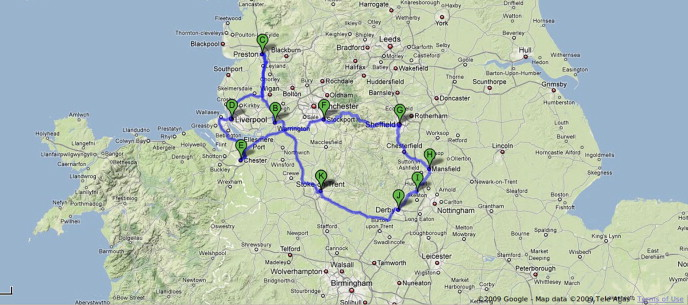
\includegraphics[keepaspectratio=true]{img/map_solution_laporte.jpg}
			\caption{Soluzione dell'istanza con un veicolo senza time window}
			\label{fig:map_laporte}
		\end{figure}


		
	\section{Risultati dell’istanza con due veicoli senza time window}
	\label{sec:istanza_due_veicoli_no_time_window}

		\begin{table}[H]
			\tiny
			\centering
			\begin{tabular}{rcccccccccc}
				\toprule
				& \rot{Chester} & \rot{Derby} & \rot{Eastwood} & \rot{Liverpool} & \rot{Mansfield} & \rot{Preston} & \rot{Sheffield} & \rot{\emph{Stockport}} & \rot{Stoke on Trent} & \rot{Warrington} \\

				\midrule

				Chester & 0 & 0 & 0 & \cellcolor{blue!25}1 & 0 & 0 & 0 & 0 & 0 & 0 \\
				Derby & 0 & 0 & 0 & 0 & 0 & 0 & 0 & 0 & \cellcolor{green!25}1 & 0 \\
				Eastwood & 0 & \cellcolor{green!25}1 & 0 & 0 & 0 & 0 & 0 & 0 & 0 & 0 \\
				Liverpool & 0 & 0 & 0 & 0 & 0 & \cellcolor{blue!25}1 & 0 & 0 & 0 & 0 \\
				Mansfield & 0 & 0 & \cellcolor{green!25}1 & 0 & 0 & 0 & 0 & 0 & 0 & 0 \\
				Preston & 0 & 0 & 0 & 0 & 0 & 0 & 0 & 0 & 0 & \cellcolor{blue!25}1 \\
				Sheffield & 0 & 0 & 0 & 0 & \cellcolor{green!25}1 & 0 & 0 & 0 & 0 & 0 \\
				\emph{Stockport} & \cellcolor{blue!25}1 & 0 & 0 & 0 & 0 & 0 & \cellcolor{green!25}1 & 0 & 0 & 0 \\
				Stoke on Trent & 0 & 0 & 0 & 0 & 0 & 0 & 0 & \cellcolor{green!25}1 & 0 & 0 \\
				Warrington & 0 & 0 & 0 & 0 & 0 & 0 & 0 & \cellcolor{blue!25}1 & 0 & 0 \\

				\bottomrule
			\end{tabular}
			\label{table:instance_2_xij}
			\caption{Valori degli $x_{ij}$ per l'istanza con due veicoli senza time window}
		\end{table}

		\begin{table}[H]
			\tiny
			\centering
			\begin{tabular}{rcccccccccc}

				\toprule
				& \rot{Chester} & \rot{Derby} & \rot{Eastwood} & \rot{Liverpool} & \rot{Mansfield} & \rot{Preston} & \rot{Sheffield} & \rot{Stockport} & \rot{Stoke on Trent} & \rot{Warrington} \\

				\midrule

				Chester & 0 & 0 & 0 & 2000 & 0 & 0 & 0 & 0 & 0 & 0 \\
				Derby & 0 & 0 & 0 & 0 & 0 & 0 & 0 & 0 & 1000 & 0 \\
				Eastwood & 0 & 1500 & 0 & 0 & 0 & 0 & 0 & 0 & 0 & 0 \\
				Liverpool & 0 & 0 & 0 & 0 & 0 & 1500 & 0 & 0 & 0 & 0 \\
				Mansfield & 0 & 0 & 2000 & 0 & 0 & 0 & 0 & 0 & 0 & 0 \\
				Preston & 0 & 0 & 0 & 0 & 0 & 0 & 0 & 0 & 0 & 1000 \\
				Sheffield & 0 & 0 & 0 & 0 & 2500 & 0 & 0 & 0 & 0 & 0 \\
				Stockport & 2500 & 0 & 0 & 0 & 0 & 0 & 3000 & 0 & 0 & 0 \\
				Stoke on Trent & 0 & 0 & 0 & 0 & 0 & 0 & 0 & 500  & 0 & 0 \\
				Warrington & 0 & 0 & 0 & 0 & 0 & 0 & 0 & 500 & 0 & 0 \\
				\bottomrule
			\end{tabular}
			\label{table:instance_2_f}
			\caption{Quantità di merce traportata $f_{ij}$ per l'istanza con due veicoli senza time window}
		\end{table}


		\begin{table}[H]
			\tiny
			\centering
			\begin{tabular}{rcccccccccc}

				\toprule
				& \rot{Chester} & \rot{Derby} & \rot{Eastwood} & \rot{Liverpool} & \rot{Mansfield} & \rot{Preston} & \rot{Sheffield} & \rot{Stockport} & \rot{Stoke on Trent} & \rot{Warrington} \\

				\midrule

				Chester & 0 & 0 & 0 & 1 & 0 & 0 & 0 & 0 & 0 & 0 \\
				Derby & 0 & 0 & 0 & 0 & 0 & 0 & 0 & 0 & 1 & 0 \\
				Eastwood & 0 & 1 & 0 & 0 & 0 & 0 & 0 & 0 & 0 & 0 \\
				Liverpool & 0 & 0 & 0 & 0 & 0 & 1 & 0 & 0 & 0 & 0 \\
				Mansfield & 0 & 0 & 1 & 0 & 0 & 0 & 0 & 0 & 0 & 0 \\
				Preston & 0 & 0 & 0 & 0 & 0 & 0 & 0 & 0 & 0 & 1 \\
				Sheffield & 0 & 0 & 0 & 0 & 1 & 0 & 0 & 0 & 0 & 0 \\
				Stockport & 1 & 0 & 0 & 0 & 0 & 0 & 1 & 0 & 0 & 0 \\
				Stoke on Trent & 0 & 0 & 0 & 0 & 0 & 0 & 0 & 1 & 0 & 0 \\
				Warrington & 0 & 0 & 0 & 0 & 0 & 0 & 0 & 1 & 0 & 0 \\

				\bottomrule
			\end{tabular}
			\label{table:instance_1_z_1}
			\caption{Valori di $z_{ij}^1$ per l'istanza con due veicoli senza time window}
		\end{table}	

		% \begin{minipage}[t]{0.49\textwidth}
		% 	\begin{table}[H]
		% 	\tiny
		% 	\centering
		% 	\label{table:instance_2_z_2}
		% 	\begin{tabular}{p{1cm} cccccccccc}

		% 		\toprule
		% 		& \rot{Chester} & \rot{Derby} & \rot{Eastwood} & \rot{Liverpool} & \rot{Mansfield} & \rot{Preston} & \rot{Sheffield} & \rot{Stockport} & \rot{Stoke on Trent} & \rot{Warrington} \\

		% 		\midrule

		% 		Chester & 0 & 0 & 0 & 0 & 0 & 0 & 0 & 0 & 0 & 0 \\
		% 		Derby & 0 & 0 & 0 & 0 & 0 & 0 & 0 & 0 & 0 & 0 \\
		% 		Eastwood & 0 & 0 & 0 & 0 & 0 & 0 & 0 & 0 & 0 & 0 \\
		% 		Liverpool & 0 & 0 & 0 & 0 & 0 & 0 & 0 & 0 & 0 & 0 \\
		% 		Mansfield & 0 & 0 & 0 & 0 & 0 & 0 & 0 & 0 & 0 & 0 \\
		% 		Preston & 0 & 0 & 0 & 0 & 0 & 0 & 0 & 0 & 0 & 0 \\
		% 		Sheffield & 0 & 0 & 0 & 0 & 0 & 0 & 0 & 0 & 0 & 0 \\
		% 		Stockport & 0 & 0 & 0 & 0 & 0 & 0 & 0 & 0 & 0 & 0 \\
		% 		Stoke on Trent & 0 & 0 & 0 & 0 & 0 & 0 & 0 & 0 & 0 & 0 \\
		% 		Warrington & 0 & 0 & 0 & 0 & 0 & 0 & 0 & 0 & 0 & 0 \\
		% 		\bottomrule
		% 	\end{tabular}
		% \end{table}
		% \end{minipage}

		\begin{table}[H]
			\tiny
			\centering
			\begin{tabular}{rc}

				\toprule
				& Tempo di Arrivo \\

				\midrule
				Chester & 0.694545 \\
				Derby & 4.48 \\
				Eastwood & 3.63636 \\
				Liverpool & 1.72182 \\
				Mansfield & 2.78364 \\
				Preston & 3.21818 \\
				Sheffield & 1.58 \\
				Stockport & 0 \\
				Stoke on Trent & 6.00545 \\
				Warrington & 4.62545 \\
				\midrule
				\textbf{Costo totale} & 181.017 € \\
				\textbf{Tourtime (Stokeontrent)} & 7.77636 ore \\
				\textbf{Tourtime (Warrington)} & 5.79818 ore \\
				\bottomrule
			\end{tabular}
			\label{table:instance_2_totale}
			\caption{Tempi di arrivo, costo totale e tourtime complessivo per l'istanza con due veicoli senza time window}
		\end{table}


	\section{Risultati dell’istanza con tre veicoli senza time window}
	\label{sec:istanza_tre_veicoli_no_time_window}


		\begin{table}[H]
			\tiny
			\centering
			\begin{tabular}{rcccccccccc}
				\toprule
				& \rot{Chester} & \rot{Derby} & \rot{Eastwood} & \rot{Liverpool} & \rot{Mansfield} & \rot{Preston} & \rot{Sheffield} & \rot{\emph{Stockport}} & \rot{Stoke on Trent} & \rot{Warrington} \\

				\midrule
				Chester & 0 & 0 & 0 & \cellcolor{blue!25}1 & 0 & 0 & 0 & 0 & 0 & 0 \\
				Derby & 0 & 0 & 0 & 0 & 0 & 0 & 0 & \cellcolor{green!25}1 & 0 & 0 \\
				Eastwood & 0 & \cellcolor{green!25}1 & 0 & 0 & 0 & 0 & 0 & 0 & 0 & 0 \\
				Liverpool & 0 & 0 & 0 & 0 & 0 & \cellcolor{blue!25}1 & 0 & 0 & 0 & 0 \\
				Mansfield & 0 & 0 & \cellcolor{green!25}1 & 0 & 0 & 0 & 0 & 0 & 0 & 0 \\
				Preston & 0 & 0 & 0 & 0 & 0 & 0 & 0 & \cellcolor{blue!25}1 & 0 & 0 \\
				Sheffield & 0 & 0 & 0 & 0 & 0 & 0 & 0 & \cellcolor{red!25}1 & 0 & 0 \\
				\emph{Stockport} & \cellcolor{blue!25}1 & 0 & 0 & 0 & \cellcolor{green!25}1 & 0 & 0 & 0 & 0 & \cellcolor{red!25}1 \\
				Stoke on Trent & 0 & 0 & 0 & 0 & 0 & 0 & \cellcolor{red!25}1 & 0 & 0 & 0 \\
				Warrington & 0 & 0 & 0 & 0 & 0 & 0 & 0 & 0 & \cellcolor{red!25}1 & 0 \\
				\bottomrule
			\end{tabular}
			\label{table:instance_3_xij}
			\caption{Valori degli $x_{ij}$ per l'istanza con tre veicoli senza time window}
		\end{table}


		\begin{table}[H]
			\tiny
			\centering
			\begin{tabular}{rcccccccccc}

				\toprule
				& \rot{Chester} & \rot{Derby} & \rot{Eastwood} & \rot{Liverpool} & \rot{Mansfield} & \rot{Preston} & \rot{Sheffield} & \rot{Stockport} & \rot{Stoke on Trent} & \rot{Warrington} \\

				\midrule

				Chester & 0 & 0 & 0 & 2100 & 0 & 0 & 0 & 0 & 0 & 0 \\
				Derby & 0 & 0 & 0 & 0 & 0 & 0 & 0 & 700 & 0 & 0 \\
				Eastwood & 0 & 1400 & 0 & 0 & 0 & 0 & 0 & 0 & 0 & 0 \\
				Liverpool & 0 & 0 & 0 & 0 & 0 & 1400 & 0 & 0 & 0 & 0 \\
				Mansfield & 0 & 0 & 2100 & 0 & 0 & 0 & 0 & 0 & 0 & 0 \\
				Preston & 0 & 0 & 0 & 0 & 0 & 0 & 0 & 700 & 0 & 0 \\
				Sheffield & 0 & 0 & 0 & 0 & 0 & 0 & 0 & 700 & 0 & 0 \\
				Stockport & 2800 & 0 & 0 & 0 & 2800 & 0 & 0 & 0 & 0 & 2800 \\
				Stoke on Trent & 0 & 0 & 0 & 0 & 0 & 0 & 1400 & 0 & 0 & 0 \\
				Warrington & 0 & 0 & 0 & 0 & 0 & 0 & 0 & 0 & 2100 & 0 \\
				\bottomrule
			\end{tabular}
			\label{table:instance_3_f}
			\caption{Quantità di merce traportata $f_{ij}$ per l'istanza con tre veicolo senza time window}
		\end{table}

		\begin{table}[H]
			\tiny
			\centering
			\begin{tabular}{rcccccccccc}

				\toprule
				& \rot{Chester} & \rot{Derby} & \rot{Eastwood} & \rot{Liverpool} & \rot{Mansfield} & \rot{Preston} & \rot{Sheffield} & \rot{Stockport} & \rot{Stoke on Trent} & \rot{Warrington} \\

				\midrule

				Chester & 0 & 0 & 0 & 1 & 0 & 0 & 0 & 0 & 0 & 0 \\
				Derby & 0 & 0 & 0 & 0 & 0 & 0 & 0 & 1 & 0 & 0 \\
				Eastwood & 0 & 1 & 0 & 0 & 0 & 0 & 0 & 0 & 0 & 0 \\
				Liverpool & 0 & 0 & 0 & 0 & 0 & 1 & 0 & 0 & 0 & 0 \\
				Mansfield & 0 & 0 & 1 & 0 & 0 & 0 & 0 & 0 & 0 & 0 \\
				Preston & 0 & 0 & 0 & 0 & 0 & 0 & 0 & 1 & 0 & 0 \\
				Sheffield & 0 & 0 & 0 & 0 & 0 & 0 & 0 & 1 & 0 & 0 \\
				Stockport & 1 & 0 & 0 & 0 & 1 & 0 & 0 & 0 & 0 & 1 \\
				Stoke on Trent & 0 & 0 & 0 & 0 & 0 & 0 & 1 & 0 & 0 & 0 \\
				Warrington & 0 & 0 & 0 & 0 & 0 & 0 & 0 & 0 & 1 & 0 \\
				\bottomrule
			\end{tabular}
			\label{table:instance_3_z_1}
			\caption{Valori di $z_{ij}^1$ per l'istanza con tre veicoli senza time window}
		\end{table}	

		% \begin{minipage}[t]{0.49\textwidth}
		% 	\begin{table}[H]
		% 	\tiny
		% 	\centering
		% 	\label{table:instance_3_z_2}
		% 	\begin{tabular}{p{1cm} cccccccccc}

		% 		\toprule
		% 		& \rot{Chester} & \rot{Derby} & \rot{Eastwood} & \rot{Liverpool} & \rot{Mansfield} & \rot{Preston} & \rot{Sheffield} & \rot{Stockport} & \rot{Stoke on Trent} & \rot{Warrington} \\

		% 		\midrule

		% 		Chester & 0 & 0 & 0 & 0 & 0 & 0 & 0 & 0 & 0 & 0 \\
		% 		Derby & 0 & 0 & 0 & 0 & 0 & 0 & 0 & 0 & 0 & 0 \\
		% 		Eastwood & 0 & 0 & 0 & 0 & 0 & 0 & 0 & 0 & 0 & 0 \\
		% 		Liverpool & 0 & 0 & 0 & 0 & 0 & 0 & 0 & 0 & 0 & 0 \\
		% 		Mansfield & 0 & 0 & 0 & 0 & 0 & 0 & 0 & 0 & 0 & 0 \\
		% 		Preston & 0 & 0 & 0 & 0 & 0 & 0 & 0 & 0 & 0 & 0 \\
		% 		Sheffield & 0 & 0 & 0 & 0 & 0 & 0 & 0 & 0 & 0 & 0 \\
		% 		Stockport & 0 & 0 & 0 & 0 & 0 & 0 & 0 & 0 & 0 & 0 \\
		% 		Stoke on Trent & 0 & 0 & 0 & 0 & 0 & 0 & 0 & 0 & 0 & 0 \\
		% 		Warrington & 0 & 0 & 0 & 0 & 0 & 0 & 0 & 0 & 0 & 0 \\
		% 		\bottomrule
		% 	\end{tabular}
		% \end{table}
		% \end{minipage}

		\begin{table}[H]
			\tiny
			\centering
			\begin{tabular}{rc}

				\toprule
				& Tempo di Arrivo \\

				\midrule
				Chester & 0.694545 \\
				Derby & 3.65273 \\
				Eastwood & 2.80909 \\
				Liverpool & 1.72182 \\
				Mansfield & 1.95636 \\
				Preston  & 3.21818 \\
				Sheffield & 4.64364 \\
				Stockport & 0 \\
				Stoke on Trent & 2.75636 \\
				Warrington & 1.17273 \\
				\midrule
				\textbf{Costo totale} & 232.976 € \\
				\textbf{Tourtime (Derby)} & 5.72364 ore \\
				\textbf{Tourtime (Preston)} & 4.95818 ore \\
				\textbf{Tourtime (Sheffield)} & 6.22364 ore \\
				\bottomrule
			\end{tabular}
			\label{table:instance_3_totale}
			\caption{Tempi di arrivo, costo totale e tourtime complessivo per l'istanza con tre veicoli senza time window}
		\end{table}

	\section{Risultati dell’istanza con due veicoli con time window}
	\label{sec:istanza_due_veicoli_con_time_window}

		\begin{table}[H]
			\tiny
			\centering
			\begin{tabular}{rcccccccccc}
				\toprule
				& \rot{Chester} & \rot{Derby} & \rot{Eastwood} & \rot{Liverpool} & \rot{Mansfield} & \rot{Preston} & \rot{Sheffield} & \rot{\emph{Stockport}} & \rot{Stoke on Trent} & \rot{Warrington} \\

				\midrule
				Chester & 0 & 0 & 0 & 0 & 0 & 0 & 0 & \cellcolor{green!25}1 & 0 & 0 \\
				Derby & 0 & 0 & \cellcolor{blue!25}1 & 0 & 0 & 0 & 0 & 0 & 0 & 0 \\
				Eastwood & 0 & 0 & 0 & 0 & \cellcolor{blue!25}1 & 0 & 0 & 0 & 0 & 0 \\
				Liverpool & \cellcolor{green!25}1 & 0 & 0 & 0 & 0 & 0 & 0 & 0 & 0 & 0 \\
				Mansfield & 0 & 0 & 0 & 0 & 0 & 0 & \cellcolor{blue!25}1 & 0 & 0 & 0 \\
				Preston & 0 & 0 & 0 & \cellcolor{green!25}1 & 0 & 0 & 0 & 0 & 0 & 0 \\
				Sheffield & 0 & 0 & 0 & 0 & 0 & 0 & 0 & \cellcolor{blue!25}1 & 0 & 0 \\
				Stockport & 0 & 0 & 0 & 0 & 0 & 0 & 0 & 0 & \cellcolor{blue!25}1 & \cellcolor{green!25}1 \\
				Stoke on Trent & 0 & \cellcolor{blue!25}1 & 0 & 0 & 0 & 0 & 0 & 0 & 0 & 0 \\
				Warrington & 0 & 0 & 0 & 0 & 0 & \cellcolor{green!25}1 & 0 & 0 & 0 & 0 \\

				\bottomrule
			\end{tabular}
			\label{table:instance_4_xij}
			\caption{Valori degli $x_{ij}$ per l'istanza con due veicoli con time window}
		\end{table}


		\begin{table}[H]
			\tiny
			\centering
			\begin{tabular}{rcccccccccc}

				\toprule
				& \rot{Chester} & \rot{Derby} & \rot{Eastwood} & \rot{Liverpool} & \rot{Mansfield} & \rot{Preston} & \rot{Sheffield} & \rot{Stockport} & \rot{Stoke on Trent} & \rot{Warrington} \\

				\midrule

				Chester & 0 & 0 & 0 & 0 & 0 & 0 & 0 & 500 & 0 & 0\\
				Derby & 0 & 0 & 2000 & 0 & 0 & 0 & 0 & 0 & 0 & 0\\
				Eastwood & 0 & 0 & 0 & 0 & 1500 & 0 & 0 & 0 & 0 & 0\\
				Liverpool & 1000 & 0 & 0 & 0 & 0 & 0 & 0 & 0 & 0 & 0\\
				Mansfield & 0 & 0 & 0 & 0 & 0 & 0 & 1000 & 0 & 0 & 0\\
				Preston & 0 & 0 & 0 & 1500 & 0 & 0 & 0 & 0 & 0 & 0\\
				Sheffield & 0 & 0 & 0 & 0 & 0 & 0 & 0 & 500 & 0 & 0\\
				Stockport & 0 & 0 & 0 & 0 & 0 & 0 & 0 & 0 & 3000 & 2500\\
				Stoke on Trent & 0 & 2500 & 0 & 0 & 0 & 0 & 0 & 0 & 0 & 0\\
				Warrington & 0 & 0 & 0 & 0 & 0 & 2000 & 0 & 0 & 0 & 0\\

				\bottomrule
			\end{tabular}
			\label{table:instance_4_f}
			\caption{Quantità di merce traportata $f_{ij}$ per l'istanza con due veicoli con time window}
		\end{table}

		\begin{table}[H]
			\tiny
			\centering
			\begin{tabular}{rcccccccccc}

				\toprule
				& \rot{Chester} & \rot{Derby} & \rot{Eastwood} & \rot{Liverpool} & \rot{Mansfield} & \rot{Preston} & \rot{Sheffield} & \rot{Stockport} & \rot{Stoke on Trent} & \rot{Warrington} \\

				\midrule

				Chester & 0 & 0 & 0 & 0 & 0 & 0 & 0 & 1 & 0 & 0 \\
				Derby & 0 & 0 & 1 & 0 & 0 & 0 & 0 & 0 & 0 & 0 \\
				Eastwood & 0 & 0 & 0 & 0 & 1 & 0 & 0 & 0 & 0 & 0 \\
				Liverpool & 1 & 0 & 0 & 0 & 0 & 0 & 0 & 0 & 0 & 0 \\
				Mansfield & 0 & 0 & 0 & 0 & 0 & 0 & 1 & 0 & 0 & 0 \\
				Preston & 0 & 0 & 0 & 1 & 0 & 0 & 0 & 0 & 0 & 0 \\
				Sheffield & 0 & 0 & 0 & 0 & 0 & 0 & 0 & 1 & 0 & 0 \\
				Stockport & 0 & 0 & 0 & 0 & 0 & 0 & 0 & 0 & 1 & 1 \\
				Stoke on Trent & 0 & 1 & 0 & 0 & 0 & 0 & 0 & 0 & 0 & 0 \\
				Warrington & 0 & 0 & 0 & 0 & 0 & 1 & 0 & 0 & 0 & 0 \\
				\bottomrule
			\end{tabular}
			\label{table:instance_4_z_1}
			\caption{Valori di $z_{ij}^1$ per l'istanza con due veicolo con time window}
		\end{table}	
	% \begin{minipage}[t]{0.49\textwidth}
		% 	\begin{table}[H]
		% 	\tiny
		% 	\centering
		% 	\label{table:instance_3_z_2}
		% 	\begin{tabular}{p{1cm} cccccccccc}

		% 		\toprule
		% 		& \rot{Chester} & \rot{Derby} & \rot{Eastwood} & \rot{Liverpool} & \rot{Mansfield} & \rot{Preston} & \rot{Sheffield} & \rot{Stockport} & \rot{Stoke on Trent} & \rot{Warrington} \\

		% 		\midrule

		% 		Chester & 0 & 0 & 0 & 0 & 0 & 0 & 0 & 0 & 0 & 0 \\
		% 		Derby & 0 & 0 & 0 & 0 & 0 & 0 & 0 & 0 & 0 & 0 \\
		% 		Eastwood & 0 & 0 & 0 & 0 & 0 & 0 & 0 & 0 & 0 & 0 \\
		% 		Liverpool & 0 & 0 & 0 & 0 & 0 & 0 & 0 & 0 & 0 & 0 \\
		% 		Mansfield & 0 & 0 & 0 & 0 & 0 & 0 & 0 & 0 & 0 & 0 \\
		% 		Preston & 0 & 0 & 0 & 0 & 0 & 0 & 0 & 0 & 0 & 0 \\
		% 		Sheffield & 0 & 0 & 0 & 0 & 0 & 0 & 0 & 0 & 0 & 0 \\
		% 		Stockport & 0 & 0 & 0 & 0 & 0 & 0 & 0 & 0 & 0 & 0 \\
		% 		Stoke on Trent & 0 & 0 & 0 & 0 & 0 & 0 & 0 & 0 & 0 & 0 \\
		% 		Warrington & 0 & 0 & 0 & 0 & 0 & 0 & 0 & 0 & 0 & 0 \\
		% 		\bottomrule
		% 	\end{tabular}
		% \end{table}
		% \end{minipage}

		\begin{table}[H]
			\tiny
			\centering
			\begin{tabular}{rc}

				\toprule
				& Tempo di Arrivo \\

				\midrule
				Chester & 13.0091 \\
				Derby  & 11.5255 \\
				Eastwood & 12.3691 \\
				Liverpool  & 11.4964 \\
				Mansfield & 14 \\
				Preston & 10 \\
				Sheffield & 15.2036 \\
				Stockport & 0 \\
				Stoke on Trent & 10 \\
				Warrington & 8.59273 \\

				\midrule
				\textbf{Costo totale} & 350.965 € \\
				\textbf{Tourtime (Chester)} & 15.0036 ore \\
				\textbf{Tourtime (Sheffield)} & 16.7836 ore \\
				\bottomrule
			\end{tabular}
			\label{table:instance_4_totale}
			\caption{Tempi di arrivo, costo totale e tourtime complessivo per l'istanza con due veicolo con time window}
		\end{table}

	\section{Risultati dell’istanza con tre veicoli con time window}
	\label{sec:istanza_tre_veicoli_con_time_window}

		\begin{table}[H]
			\tiny
			\centering
			\begin{tabular}{rcccccccccc}
				\toprule
				& \rot{Chester} & \rot{Derby} & \rot{Eastwood} & \rot{Liverpool} & \rot{Mansfield} & \rot{Preston} & \rot{Sheffield} & \rot{\emph{Stockport}} & \rot{Stoke on Trent} & \rot{Warrington} \\

				\midrule
				Chester & 0 & 0 & 0 & 0 & 0 & 0 & 0 & \cellcolor{green!25}1 & 0 & 0 \\
				Derby & 0 & 0 & 0 & 0 & 0 & 0 & 0 & \cellcolor{red!25}1 & 0 & 0 \\
				Eastwood & 0 & 0 & 0 & 0 & \cellcolor{blue!25}1 & 0 & 0 & 0 & 0 & 0 \\
				Liverpool & \cellcolor{green!25}1 & 0 & 0 & 0 & 0 & 0 & 0 & 0 & 0 & 0 \\
				Mansfield & 0 & 0 & 0 & 0 & 0 & 0 & \cellcolor{blue!25}1 & 0 & 0 & 0 \\
				Preston & 0 & 0 & 0 & \cellcolor{green!25}1 & 0 & 0 & 0 & 0 & 0 & 0 \\
				Sheffield & 0 & 0 & 0 & 0 & 0 & 0 & 0 & \cellcolor{blue!25}1 & 0 & 0 \\
				Stockport & 0 & 0 & \cellcolor{blue!25}1 & 0 & 0 & \cellcolor{green!25}1 & 0 & 0 & 0 & \cellcolor{red!25}1 \\
				Stoke on Trent & 0 & \cellcolor{red!25}1 & 0 & 0 & 0 & 0 & 0 & 0 & 0 & 0 \\
				Warrington & 0 & 0 & 0 & 0 & 0 & 0 & 0 & 0 & \cellcolor{red!25}1 & 0 \\
				\bottomrule
			\end{tabular}
			\label{table:instance_5_xij}
			\caption{Valori degli $x_{ij}$ per l'istanza con tre veicoli con time window}
		\end{table}


		\begin{table}[H]
			\tiny
			\centering
			\begin{tabular}{rcccccccccc}

				\toprule
				& \rot{Chester} & \rot{Derby} & \rot{Eastwood} & \rot{Liverpool} & \rot{Mansfield} & \rot{Preston} & \rot{Sheffield} & \rot{Stockport} & \rot{Stoke on Trent} & \rot{Warrington} \\

				\midrule

				Chester & 0 & 0 & 0 & 0 & 0 & 0 & 0 & 700  & 0 & 0 \\
				Derby & 0 & 0 & 0 & 0 & 0 & 0 & 0 & 700 & 0 & 0 \\
				Eastwood & 0 & 0 & 0 & 0 & 2100 & 0 & 0 & 0  & 0 & 0 \\
				Liverpool & 1400 & 0 & 0 & 0 & 0 & 0 & 0 & 0 & 0 & 0 \\
				Mansfield & 0 & 0 & 0 & 0 & 0 & 0 & 1400 & 0 & 0 & 0 \\
				Preston & 0 & 0 & 0 & 2100 & 0 & 0 & 0 & 0  & 0 & 0 \\
				Sheffield & 0 & 0 & 0 & 0 & 0 & 0 & 0 & 700 & 0 & 0 \\
				Stockport & 0 & 0 & 2800 & 0 & 0 & 2800 & 0 & 0 & 0 & 2800 \\
				Stoke on Trent & 0 & 1400 & 0 & 0 & 0 & 0 & 0 & 0  & 0 & 0 \\
				Warrington & 0 & 0 & 0 & 0 & 0 & 0 & 0 & 0 & 2100 & 0 \\

				\bottomrule
			\end{tabular}
			\label{table:instance_5_f}
			\caption{Quantità di merce traportata $f_{ij}$ per l'istanza con tre veicoli con time window}
		\end{table}

		\begin{table}[H]
			\tiny
			\centering
			\begin{tabular}{rcccccccccc}

				\toprule
				& \rot{Chester} & \rot{Derby} & \rot{Eastwood} & \rot{Liverpool} & \rot{Mansfield} & \rot{Preston} & \rot{Sheffield} & \rot{Stockport} & \rot{Stoke on Trent} & \rot{Warrington} \\

				\midrule

				Chester & 0 & 0 & 0 & 0 & 0 & 0 & 0 & 1 & 0 & 0 \\
				Derby & 0 & 0 & 0 & 0 & 0 & 0 & 0 & 1 & 0 & 0 \\
				Eastwood & 0 & 0 & 0 & 0 & 1 & 0 & 0 & 0 & 0 & 0 \\
				Liverpool & 1 & 0 & 0 & 0 & 0 & 0 & 0 & 0 & 0 & 0 \\
				Mansfield & 0 & 0 & 0 & 0 & 0 & 0 & 1 & 0 & 0 & 0 \\
				Preston & 0 & 0 & 0 & 1 & 0 & 0 & 0 & 0 & 0 & 0 \\
				Sheffield & 0 & 0 & 0 & 0 & 0 & 0 & 0 & 1 & 0 & 0 \\
				Stockport & 0 & 0 & 1 & 0 & 0 & 1 & 0 & 0 & 0 & 1 \\
				Stoke on Trent & 0 & 1 & 0 & 0 & 0 & 0 & 0 & 0 & 0 & 0 \\
				Warrington & 0 & 0 & 0 & 0 & 0 & 0 & 0 & 0 & 1 & 0 \\
				\bottomrule
			\end{tabular}
			\label{table:instance_5_z_1}
			\caption{Valori di $z_{ij}^1$ per l'istanza con tre veicoli con time window}
		\end{table}	
		% \begin{minipage}[t]{0.49\textwidth}
		% 	\begin{table}[H]
		% 	\tiny
		% 	\centering
		% 	\label{table:instance_3_z_2}
		% 	\begin{tabular}{p{1cm} cccccccccc}

		% 		\toprule
		% 		& \rot{Chester} & \rot{Derby} & \rot{Eastwood} & \rot{Liverpool} & \rot{Mansfield} & \rot{Preston} & \rot{Sheffield} & \rot{Stockport} & \rot{Stoke on Trent} & \rot{Warrington} \\

		% 		\midrule

		% 		Chester & 0 & 0 & 0 & 0 & 0 & 0 & 0 & 0 & 0 & 0 \\
		% 		Derby & 0 & 0 & 0 & 0 & 0 & 0 & 0 & 0 & 0 & 0 \\
		% 		Eastwood & 0 & 0 & 0 & 0 & 0 & 0 & 0 & 0 & 0 & 0 \\
		% 		Liverpool & 0 & 0 & 0 & 0 & 0 & 0 & 0 & 0 & 0 & 0 \\
		% 		Mansfield & 0 & 0 & 0 & 0 & 0 & 0 & 0 & 0 & 0 & 0 \\
		% 		Preston & 0 & 0 & 0 & 0 & 0 & 0 & 0 & 0 & 0 & 0 \\
		% 		Sheffield & 0 & 0 & 0 & 0 & 0 & 0 & 0 & 0 & 0 & 0 \\
		% 		Stockport & 0 & 0 & 0 & 0 & 0 & 0 & 0 & 0 & 0 & 0 \\
		% 		Stoke on Trent & 0 & 0 & 0 & 0 & 0 & 0 & 0 & 0 & 0 & 0 \\
		% 		Warrington & 0 & 0 & 0 & 0 & 0 & 0 & 0 & 0 & 0 & 0 \\
		% 		\bottomrule
		% 	\end{tabular}
		% \end{table}
		% \end{minipage}

		\begin{table}[H]
			\tiny
			\centering
			\begin{tabular}{rc}

				\toprule
				& Tempo di Arrivo \\

				\midrule
				Chester & 13.0091 \\
				Derby & 11.5255 \\
				Eastwood & 12 \\
				Liverpool & 11.4964 \\
				Mansfield & 14 \\
				Preston  & 10 \\
				Sheffield & 15.2036 \\
				Stockport & 0 \\
				Stoke on Trent & 10 \\
				Warrington & 8 \\


				\midrule
				\textbf{Costo totale} & 491.723€ \\
				\textbf{Tourtime (Chester)} & 15.0036 ore \\
				\textbf{Tourtime (Derby)} & 13.5964 ore \\
				\textbf{Tourtime (Sheffield)} & 16.7836 ore \\
				\bottomrule
			\end{tabular}
			\label{table:instance_5_totale}
			\caption{Tempi di arrivo, costo totale e tourtime complessivo per l'istanza con tre veicoli con time window}
		\end{table}
